\chapter{Statistické přehledy v reálném čase a vizualizační engine}
\label{ch:visualization}

V této kapitole se stručně popisuje problematika zobrazování surových astronomických dat a architektura vizualizačního subsystému. Cílem navrženého řešení je poskytnout uživateli okamžitou vizuální odezvu při procházení rozsáhlých souborových sad, což vyžaduje specifické optimalizace na úrovni softwaru i grafického hardwaru.

\section{Nelineární transformace dynamického rozsahu}
Surová data z digitálních snímačů alokují většinu užitečného signálu těsně nad úrovní šumu pozadí (viz Obrázek \ref{fig:histogram}, kde levá část (černá barva) představuje šum a pravá sestupná hrana (červená barva) obsahuje užitečná data). V důsledku tohoto vysokého dynamického rozsahu se lineární obraz při běžném zobrazení jeví jako téměř zcela černý. Pro účely lidského vyhodnocení je nutné aplikovat nelineární transformaci midtonů (\textit{Screen Transfer Function}), jejíž matematický model byl převzat z astronomického softwaru PixInsight\footnote{\url{https://pixinsight.com/}} a adaptován pro potřeby navrženého systému\footnote{\url{https://pixinsight.com/forum/index.php?threads/programmatic-way-to-do-an-stf-autostretch.6659/}}.

\begin{figure}[h] 
    \centering 
    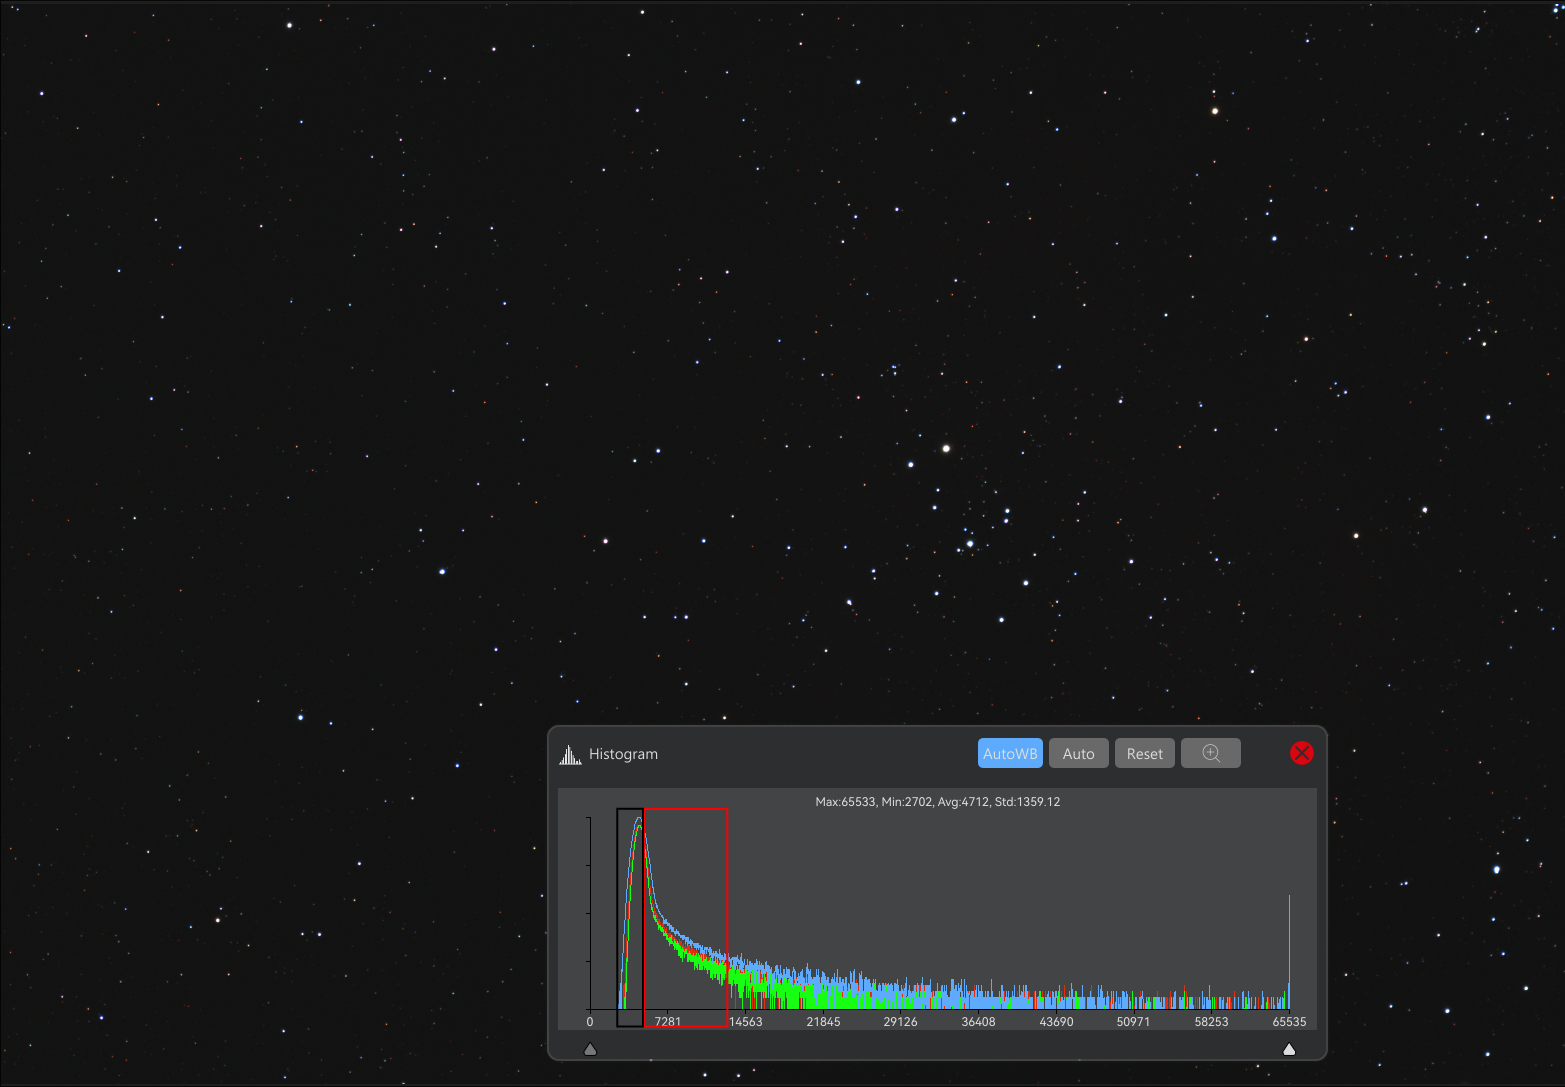
\includegraphics[width=0.78\textwidth]{assets/histogram.png} 
    \caption{Zobrazení histogramu před nelineární transformací} 
    \label{fig:histogram} 
\end{figure}

Z důvodu úspory výpočetního času systém neanalyzuje miliony pixelů každého snímku, ale provádí statistické vzorkování (analýzu každého stého pixelu). Z tohoto vzorku se vypočítává robustní mediánová absolutní odchylka (\ac{MAD}), která slouží k přesnému odhadu šumu pozadí bez zkreslení jasnými hvězdami. Následně se stanovují ořezové body pro nelineární roztažení histogramu. Systém podporuje režim propojených barevných kanálů pro zachování barevné věrnosti i režim nezávislých kanálů, který automaticky eliminuje silné barevné závoje způsobené světelným znečištěním.

\section{Hardwarová akcelerace vykreslování}
Opakovaný přepočet nelineárního strečinku na úrovni \acs{CPU} při každé změně parametrů nebo při rychlém přepínání snímků by vedl k neakceptovatelným latencím rozhraní. Výpočetní jádro proto surová data pouze normalizuje a předává je do prezentační vrstvy ve formě čistých textur. Výsledný efekt této transformace a okamžitého zobrazení skrytých detailů v uživatelském rozhraní je znázorněn na Obrázku~\ref{fig:autostf_preview}.

\begin{figure}[h]
    \centering
    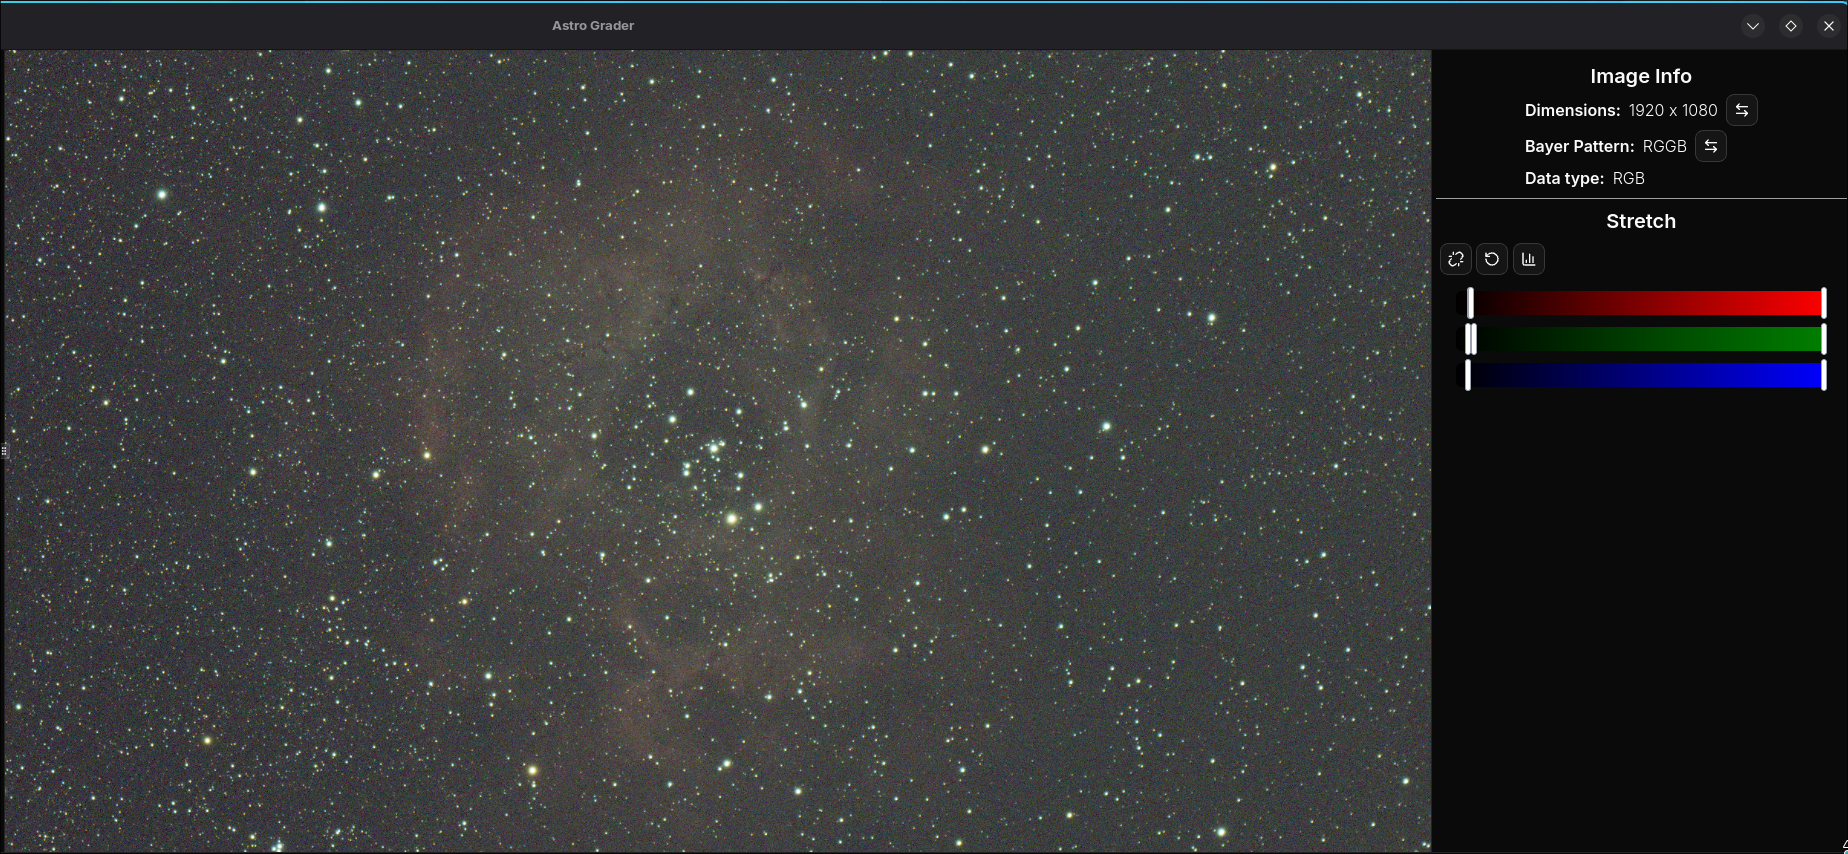
\includegraphics[width=0.78\textwidth]{assets/stretched.png}
    \caption{Vizualizace astronomického snímku po aplikaci automatické nelineární transformace jasu (AutoSTF).}
    \label{fig:autostf_preview}
\end{figure}

Vlastní nelineární transformace jasu a mapování histogramu probíhá v reálném čase přímo na grafické kartě počítače. K tomuto účelu se využívají vlastní \ac{WebGL} fragment shadery. Výpočetní zátěž se tím přenáší z procesoru na vysoce paralelní architekturu GPU, což umožňuje naprosto plynulé procházení a renderování snímků s nulovou latencí uživatelského rozhraní.